% \section{Process view: workflows}
% \label{sec:Workflows}

LArSoft tools can be sequenced and combined to define complete workflows.
The typical usage is aligned to three main types of ``standard'' workflows: % (\cref{fig:LArSoftProcessingChain}):
\begin{enumerate}
  \item simulation
  \item reconstruction
  \item analysis
\end{enumerate}
where the first step, simulation, is of course skipped when processing real detector data.
% \begin{figure}
%   \centering
%   \includegraphics[width=\textwidth]{figures/LArSoftWorkflows}
%   \caption{\label{fig:LArSoftProcessingChain}Typical workflow sequence in liquid argon TPC analysis. Each block represents a workflow.}
%   % REMOVE DIAGRAM
% \end{figure}
LArSoft does not directly define these processing chains.
Rather, it inherits the flexibility from the \emph{art} framework,
which provides users with the flexibility of choosing and arranging processing modules at will.
%, with the only limitation that each module
% must be provided with all the information it needs to operate.
% A module can be executed multiple times, with different configurations.\\
Thus, the Experiments define the steps of each workflow according to their needs.
Still, these needs are fairly shared,
and it is possible to characterize a ``typical'' chain for each workflow.


\subsection{Simulation workflow}
\label{ssec:Workflows:Simulation}

The purpose of a simulation workflow is to describe a realistic response of
the detectors to a known physics event (``truth'').
Since the result of the simulation should be equivalent to the output of the detectors,
this result is represented in both cases by the same data structures.

The main results of this workflow are:
\begin{itemize}
   \item data products representing the detector response (\eg \ClassName{raw::RawDigit} and \ClassName{raw::OpDetWaveform})
   \item data products representing the simulated physics (\eg \ClassName{simb::MCTruth}, \ClassName{simb::MCParticle})
\end{itemize}

\begin{figure}
   \centering
   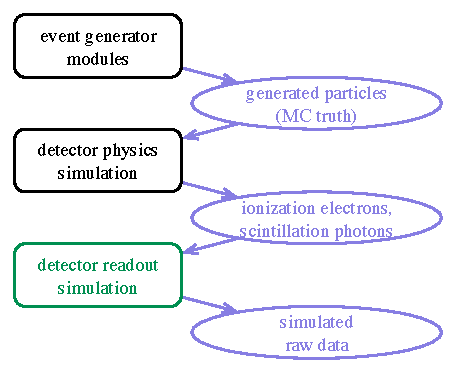
\includegraphics{figures/LArSoftSimulationWorkflow}
   \caption{\label{fig:LArSoftSimulationWorkflow}
      A typical LArSoft simulation workflow.
      Blocks represent operations and ellipse represents data.
      Block colour coding follows \cref{fig:LArSoftRelations}.
   }
\end{figure}
The complete simulation chain is illustrated in \cref{fig:LArSoftSimulationWorkflow}.
The process is typically divided in three steps:
\begin{enumerate}
   \item event generation
   \item detector physics simulation
   \item detector readout simulation
      \begin{itemize}
         \item TPC: signal on the wires
         \item optical detector(s)
         \item ``auxiliary'' detectors (\eg scintillator pads)
      \end{itemize}
\end{enumerate}

\begin{figure}
   \centering
   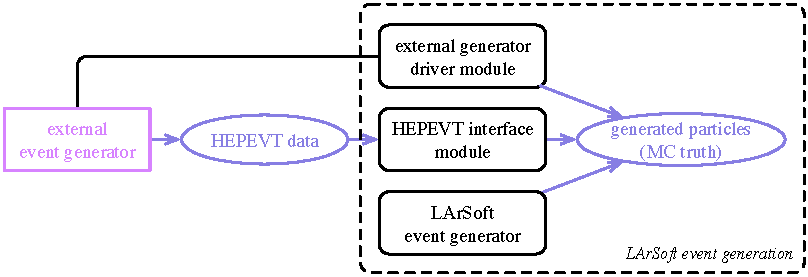
\includegraphics{figures/LArSoftEventGeneration}
   \caption{\label{fig:LArSoftEventGeneration}
      Event generation workflow.
      Blocks represent operations and ellipses represent data.
      Block colour coding follows \cref{fig:LArSoftRelations}.
      The dashed line encompasses the part of the workflow driven via LArSoft configuration.
   }
\end{figure}
The physics event can be generated by an external program or library (\cref{fig:LArSoftEventGeneration}).
LArSoft can interface directly to generators that offer API, through a specific driver module.
Currently driver modules are offered to work
with GENIE generator (neutrino interactions) and CRY (cosmic rays).
LArSoft can also read events stored in HEPEVT format.
In addition, LArSoft provides built-in generators for single particles,
Argon nucleus decays, and more.

\begin{figure}
   \centering
   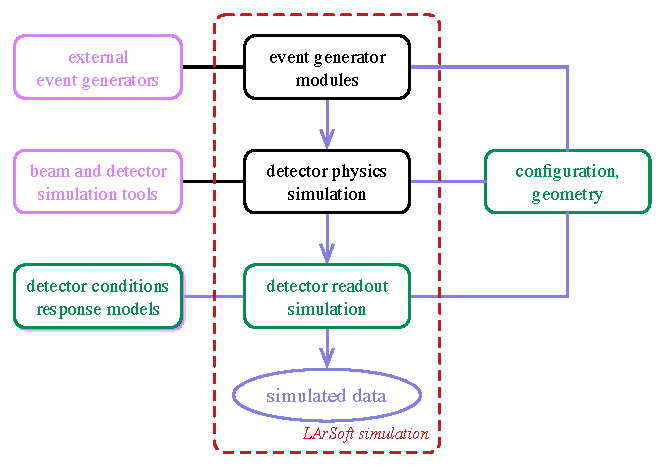
\includegraphics{figures/LArSoftSimulationComponents}
   \caption{\label{fig:LArSoftSimulationRelations}
      Components involved in simulation and their relation.
      Blocks represent operations and ellipse represents data.
      Lines represent communication between components: via data transfer (purple lines) and via API (black lines). 
      Block colour coding follows \cref{fig:LArSoftRelations}.
      The encircled area maps the simulation workflow illustrated in \cref{fig:LArSoftSimulationWorkflow}.
   }
\end{figure}
The detector physics simulation includes interaction of 
generated particles with the detector,
and transportation to the readout of produced photons and electrons.
This part of the simulation currently relies on \GEANT for the interaction of particles with matter.
Photon and electron transportation is implemented in built-in code.
Detector parameters (\eg, the intensity of the electric field)
can be acquired from the job configuration or from a Experiment database.

The last step transforms the physics information, electrons and photons,
into digitized detector response,
including the simulation of electronics noise and shaping.
This is typically implemented with experiment-specific code,
and separately for each sub-detector type.


\subsection{Reconstruction workflow}
\label{ssec:Workflows:Reconstruction}

The reconstruction phase produces standard physics objects describing the physics event.
Reconstruction delivers objects with different level of sophistication,
as for example hits describing localized charge deposition as detected on a wire,
down to a complete hierarchy of three-dimensional tracks.
These objects are handed over for further analysis.
\begin{figure}
   \centering
   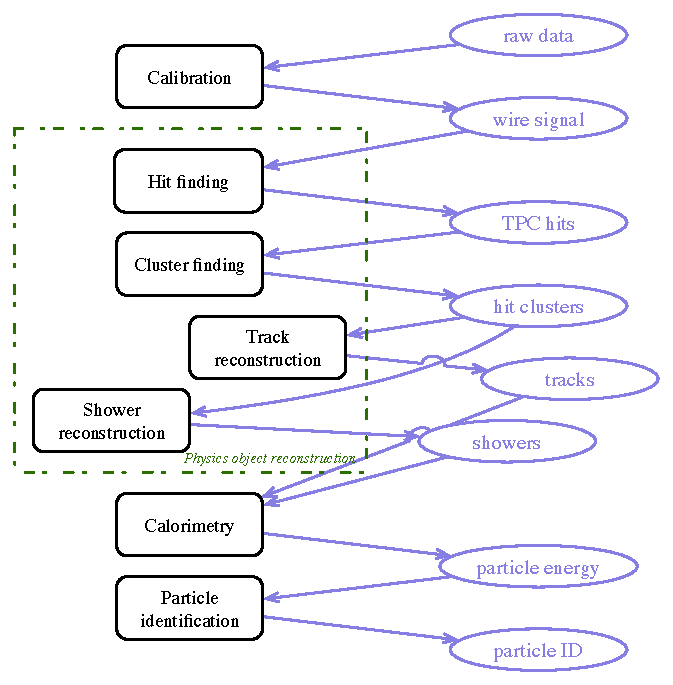
\includegraphics{figures/LArSoftReconstructionWorkflow}
   \caption{\label{fig:LArSoftReconstruction}
      A typical LArSoft reconstruction workflow.
      The red contour delimits the components within LArSoft toolkit,
      and the green one encloses the reconstruction of basic physics ojects.
      Blocks represent software and ellipses represent data.
}
\end{figure}
Through the workflow, detector and data acquisition parameters
can be acquired from Experiment databases.

Many possible reconstruction strategies are possible.
LArSoft allows them to be applied indifferently to data produced by a real detector or simulated.
Support is planned for mixing the two types of sources together.
The more ``traditional'' one (\cref{fig:LArSoftReconstruction}) proceeds through:
\begin{enumerate}
  \item calibration of the signals, noise suppression and removal of electronics distortions;
  \item independent reconstruction of charge deposition on each TPC wire (\emph{hits});
  \item definition of \emph{clusters} from hits lying on the same wire plane;
  \item combination of clusters from different planes in trajectories (\emph{tracks}) and particle cascades (\emph{showers});
  \item identification of interaction points (\emph{vertices});
  \item hierarchal connection of them into \emph{particle flow} structures. Many options are implemented in LArSoft for each.
\end{enumerate}
Different algorithms can be chosen to perform each of these steps.
Any external library that utilizes LArSoft data classes to receive inputs
and deliver results is also fully interchangeable with the algorithms implemented in LArSoft.
A noticeable example is the \Pandora pattern recognition toolkit,
that accepts LArSoft hits as input and can present its results in the form of LArSoft clusters,
tracks and particle flow objects.

This workflow is extremely simple and factorizes the process in highly independent steps.
Alternative workflows can and have been developed.\\
For example, a derivation of the workflow described above consists in a complete
first pass tuned for reconstruction and subsequent identification of background
objects (mostly cosmic rays); in their elimination at the level of hits;
and in a second pass tuned for reconstruction of neutrino interactions.\\
Other approaches include direct track reconstruction without clustering;
direct clustering from calibrated or uncalibrated channel signals by image processing algorithms,
bypassing the construction of hits;
a quick, preliminary track reconstruction
followed by a complete reconstruction utilizing the first result to better direct the algorithms;
inverting the order of track and vertex finding;
and more.

LArSoft and \ART modularity supports any acyclic workflows,
with any predetermined number of (potentially optional) steps.
It does not accommodate cyclic workflows.


\subsection{Analysis workflow}
\label{ssec:Workflows:Analysis}

Analysis workflows are the most vaguely defined,
due in part to the more diverse goals,
and partly to the fact that in this relatively early stage the Experiments
have devoted most of the time to simulation and reconstruction.
No prototype analysis workflow has emerged yet.

The calibration of energy deposited in liquid argon by interacting particles
and their identification as specific types (\eg, muons, protons, etc.)
have been classified sometimes as ``analysis'', sometimes as ``reconstruction''.
Another common analysis task is evaluation of reconstruction performances
and comparison between different algorithms and strategies.

Calibration activities, for example pedestal analysis,
characterization of argon purity, mapping of the electric field,
also fall in this category and they are ideal candidates for the standardization of workflows.
